\section{SpatialVLA Within-Call Edits: Path and Discovery Pilot}
\label{sec:svla}
\paragraph{Model and decoding.}
\begin{itemize}
\item \textbf{Model.} We use \texttt{spatialvla-4b-224-sft-fractal} (SigLIP + Gemma~2; transformers 4.47.0; bf16; eager attention) with its official processor and the official SimplerEnv adapter. The adapter uses 224$\times$224 inputs, predicts every control step, ensembles over 4 chunks (temperature $-0.8$) and applies a sticky gripper.
\item \textbf{Output format.} Every natural output in this study has 13 tokens: 4 actions $\times$ (translation, rotation, gripper), then EOS.
\item \textbf{Action coding.} Translation tokens are 4,096 spherical bins and rotation tokens are $16^3$ Euler bins; the gripper takes 2 values.
\item \textbf{Response space.} The official decoder maps tokens to normalized actions before unnormalization. The six motion components of $a_3,a_4$ form the response space. Normalized Euler differences are not geodesic rotations, and these command differences are not end-effector motion.
\item \textbf{Parser.} The official parser zero-pads short outputs and clips out-of-range ids. We therefore check token types ourselves and never pad.
\end{itemize}

\paragraph{Adapter path.}
\begin{itemize}
\item \textbf{Mechanics.} The adapter prefills the prompt once with a HybridCache of length $P{+}256$, as \texttt{generate} does, and then feeds one action token per forward pass. The prompt keeps the official bidirectional mask, and generated or forced tokens are causal. Forced conditioning tokens never enter the prompt.
\item \textbf{Evaluation path.} In the transformers version used, \texttt{generate} stores its cache on the model and reuses it whenever it is long enough. In the discovery pilot, calls made after longer move\_near prompts therefore ran with a larger cache:
  \begin{itemize}
  \item the record-time official output differed from the collection-time output in 7/105 observations;
  \item self-patch identity failed in 4/105 observations.
  \end{itemize}
\item \textbf{Fix and diagnosis.} All reported SpatialVLA results use the official model and processor \emph{with a fresh cache per call}. In a fresh-process diagnostic all affected observations were consistent; deterministic kernels changed tokens and were not used. Three residual first-attempt disagreements were not isolated, and we do not attribute all differences to bf16 arithmetic.
\item \textbf{Logit-level parity.}
  \begin{itemize}
  \item The adapter's natural decoding differs from the official logits by at most 0.125, with no token change.
  \item Self-patch continuation logits are bitwise equal in validation, in the discovery pilot and in the follow-up.
  \item In the drawer task they differ by at most 0.5, again with no token change.
  \end{itemize}
\end{itemize}

\paragraph{Discovery pilot (v01).}
\begin{itemize}
\item \textbf{Path checks.} Self-patch was token-identical in 12/12 validation observations and 105/105 pilot observations (coke: 25 new layouts; move\_near: all 10 layouts, reused).
\item \textbf{Donors.} The first joint-valid donor among four samples was used; 41 observations had none. Of 420 samples, 297 reproduced a natural action.
\item \textbf{Pre-specified primary analysis (distance-matched).} Only 7 observations qualified (6 coke layouts and 1 move\_near layout): $\Delta=0.084$, two-task interval not computed.
\item \textbf{Secondary analysis (all 64 joint-valid observations).} $\Delta=0.070$ $[0.044,0.100]$. On average the L donors were farther than the O donors, so this result is partly confounded by donor distance and is not promoted to a primary result.
\item \textbf{Reselection check.} Among the 420 discovery-pilot samples, any distance-matched candidate existed for only 16 observations in 15 layouts (2 move\_near). This motivated a new, pre-registered donor rule rather than reselection.
\end{itemize}

\section{SpatialVLA Matched Follow-up (v02)}
\label{sec:svla2}
\paragraph{Design (pre-registered before any v02 intervention output).}
\begin{itemize}
\item \textbf{Layouts.} coke uses the first 25 layouts from a survey of seeds 4000--4099 that are disjoint from all discovery-pilot and validation layouts. move\_near reuses the same 10 layouts, seeds and instructions.
\item \textbf{Observations.} Images before natural generation calls 2, 6 and 10 (105 observations). None is identical to a discovery-pilot input.
\item \textbf{Donor rule.} At most 64 sequential official samples per observation ($T{=}0.7$, top-$p$ 1, top-$k$ 0; seeds hashed from the observation id). The first sample that is joint-valid and satisfies $0.8\le d_L/d_O\le1.25$ is used for O, L and OL. If none of the 64 qualifies, the observation is MATCHED\_SOURCE\_MISSING; there is no further search.
\item \textbf{Analysis.} Equal-weight layouts within each task, equal-weight tasks, and a layout bootstrap within tasks (10,000 resamples, seed 20261023).
\item \textbf{Relation to the discovery pilot.} The donor rule and observation calls differ from the discovery pilot, so the two are separate experiments and are never pooled. Because tasks and the move\_near layouts are reused, this is not an independent task-generalization test.
\end{itemize}

\begin{table}[h]
\centering\small
\caption{\textbf{SpatialVLA follow-up denominators} (observations; layouts in parentheses).}
\label{tab:svla2flow}
\begin{tabular}{@{}lrrr@{}}\toprule
Stage & coke & move\_near & Total\\\midrule
Panel layouts & 25 & 10 (reused) & 35\\
Collected observations (calls 2/6/10) & 75 & 30 & 105\\
Valid natural output (12 typed tokens + EOS) & 75 & 30 & 105\\
Path checks pass (official = collection = adapter; R tokens and EOS) & 75 & 30 & 105\\
Matched donor within 64 samples & 55 & 14 & 69\\
Analyzed (valid O/L/OL continuations) & 55 (25) & 14 (9) & 69 (34)\\\bottomrule
\end{tabular}
\end{table}

\paragraph{Sources and coverage.}
\begin{itemize}
\item \textbf{Samples.} 3,243 samples were generated (median 22 per observation). Of these, 2,710 were rejected for zero distance (they reproduced a natural action), 396 for a ratio outside $[0.8,1.25]$ and 68 for a gripper mismatch; 69 were selected.
\item \textbf{Donor distance.} Donor distances are balanced: mean $d_L=0.054$ vs.\ $d_O=0.053$, with ratio quartiles 0.93/1.02/1.16.
\item \textbf{Coverage.} The design target was at least 15 coke and 8 move\_near matched layouts; the run reached 25 and 9.
\item \textbf{Smoke check.} Coke and move\_near observations at call 0 passed all path checks; they are not analyzed.
\end{itemize}

\begin{table}[h]
\centering\small
\caption{\textbf{SpatialVLA follow-up results} (normalized action distance; 95\% layout-bootstrap intervals; 69 observations, 34 layouts).}
\label{tab:svla2res}
\begin{tabular}{@{}lrr@{}}\toprule
Quantity & Estimate & 95\% interval\\\midrule
$\Delta=E_L-E_O$ (primary, two tasks) & 0.048 & $[0.026,0.072]$\\
\ coke (25 layouts) / move\_near (9 layouts) & 0.042 / 0.054 & $[0.015,0.070]$ / $[0.018,0.093]$\\
$E_L$ / $E_O$ & 0.070 / 0.022 & \\
$\Delta$, same change-type pattern at $a_1$ and $a_2$ (48 obs.) & 0.048 & $[0.019,0.079]$\\
$a_3$: $E_L$ / $E_O$; $a_4$: $E_L$ / $E_O$ & 0.068 / 0.027; 0.072 / 0.017 & \\
translation: $E_L$ / $E_O$; rotation: $E_L$ / $E_O$ & 0.076 / 0.020; 0.065 / 0.024 & \\
$D(OL,L)$ (direct) & 0.021 & $[0.012,0.030]$\\
$J=E_{OL}-E_O-E_L$ (descriptive) & $-0.024$ & $[-0.040,-0.011]$\\
gripper change rate in $a_3,a_4$: L / O / OL & 0.082 / 0.053 / 0.067 & \\\bottomrule
\end{tabular}
\end{table}

\paragraph{Reading the follow-up results.}
\begin{itemize}
\item \textbf{Change rates.} The latest edit changed the continuation tokens in 56/69 observations, the older edit in 27/69. In 11 of the 69 observations, $\Delta<0$.
\item \textbf{Older position.} $D(OL,L)>0$ shows that the older position is not irrelevant.
\item \textbf{Interaction.} $J$ is a descriptive interaction; it is not evidence of additivity or of its absence.
\item \textbf{Scope.} These are command-level responses with the intermediate action fixed. They were not executed, and they are not success effects.
\end{itemize}

\begin{figure}[h]
\centering
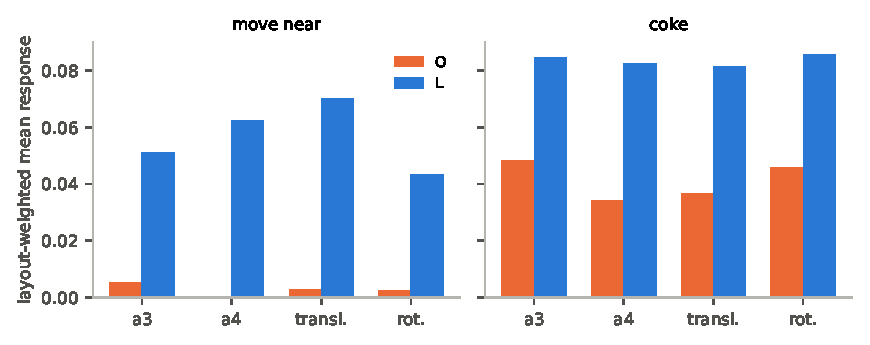
\includegraphics[width=0.75\textwidth]{fig_svla_v02_components.pdf}\\
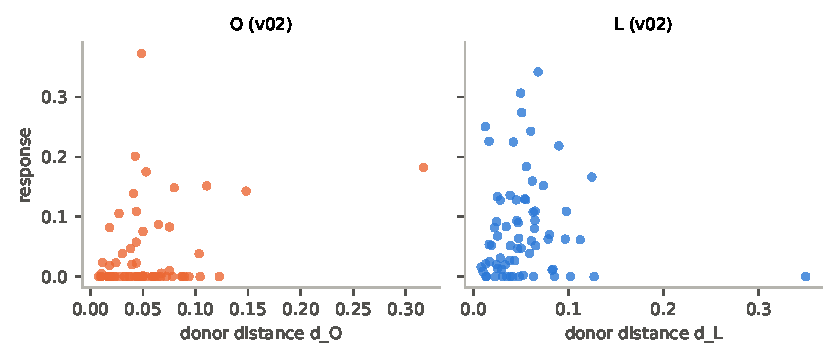
\includegraphics[width=0.6\textwidth]{fig_svla_v02_donor_distance.pdf}
\caption{\textbf{SpatialVLA follow-up: responses by continuation step and component (top) and against donor distance (bottom).} Layout-weighted means; normalized action units.}
\label{fig:svla2comp}
\end{figure}

\section{Supplementary SpatialVLA Task: Open Drawer}
\label{sec:svladrawer}
\paragraph{Task selection.}
\begin{itemize}
\item \textbf{Order checked.} Open drawer, then close drawer.
\item \textbf{Selected task.} \texttt{google\_robot\_open\_drawer} (\texttt{OpenDrawerCustomInScene-v0}).
\item \textbf{Why compatible.} It uses the same Google-robot embodiment, camera path, adapter, checkpoint and normalization, and needs no training. Selection did not use success rates or effects.
\end{itemize}

\paragraph{Panel.}
\begin{itemize}
\item \textbf{Layouts.} The cabinet is fixed; the robot pose and the target drawer vary. A layout is identified by robot and articulation poses plus the instruction. The panel was fixed as the first 20 unique layouts in seeds 5000--5099 (69 unique in total), with calls 2/6/10.
\item \textbf{Collection.} Software rendering of this scene takes about 2.2\,s per step. The first attempt was still collecting after 20.8 GPU-minutes when the process ended: it had collected 44 observations from 16 layouts and produced no intervention outputs.
\item \textbf{Amendment.} An amendment made before any intervention output reused these 44 observations as lossless images. The collection-time output check is therefore unavailable for them; all other path checks ran.
\end{itemize}

\paragraph{Results.}
\begin{itemize}
\item \textbf{Path checks.} Self-patch tokens and EOS were identical in 44/44 observations, and adapter parity held in 44/44.
\item \textbf{Donors.} A matched donor was found within 64 samples for 35/44 observations (15 layouts). Of 1,053 samples, 792 were rejected for zero distance and 226 for the ratio.
\item \textbf{Effect.} $\Delta=0.145$ $[0.091,0.210]$, with $E_L=0.183$ and $E_O=0.039$. Donor distances are balanced (0.100 vs.\ 0.101). $D(OL,L)=0.043$ $[0.020,0.067]$ and $J=-0.057$ $[-0.089,-0.030]$ (descriptive).
\item \textbf{Scope.} This is a single task with a layout-conditional interval, and it is not pooled with the two-task estimand.
\end{itemize}

\begin{figure}[h]
\centering
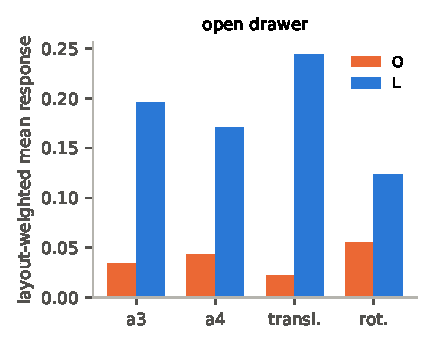
\includegraphics[width=0.45\textwidth]{fig_svla_drawer_components.pdf}\hfill
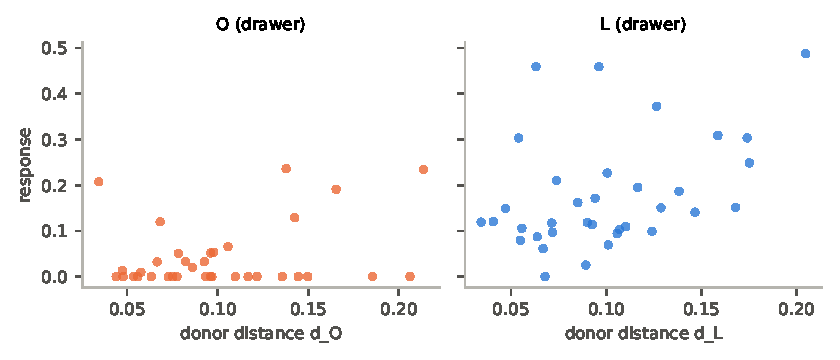
\includegraphics[width=0.52\textwidth]{fig_svla_drawer_donor_distance.pdf}
\caption{\textbf{Open-drawer supplementary task:} responses by step and component (left) and against donor distance (right).}
\label{fig:svladrawer}
\end{figure}
